% \Huge

\section{Perturbation Theory}

\todo[inline]{Give a brief introduction to the use of Perturbation theory to study the evolution of structure. Present advatages and shortcomings}

\todo[inline]{This could be merged with the next section.}
\section{Linear vs Non-Linear Collapse}

\todo[inline]{Talk about the Linear regime of collapse versus the non-linear regime. Present the difficulty of constructing analytical models of non-linear collapse. Motivate our use of simulations as well as our desire to get back to the linear regime for reconstruction.}

\todo[inline]{Add images of the velocity field here}

\section{The Zeldovich Approximation}

\todo[inline]{Introduce the theory of the Zeldovich Approximation and motivate its use (+ background).}

\section{Reconstruction (BAO)}

\todo[inline]{Finally link everything with an overview of Reconstruction techniques and how our work fits into the modern context.}

\todo[inline]{Showcase the BAO reconstruction.}

\begin{figure}
    \centering
    %\hspace*{\fill}
    \subfloat[]{
      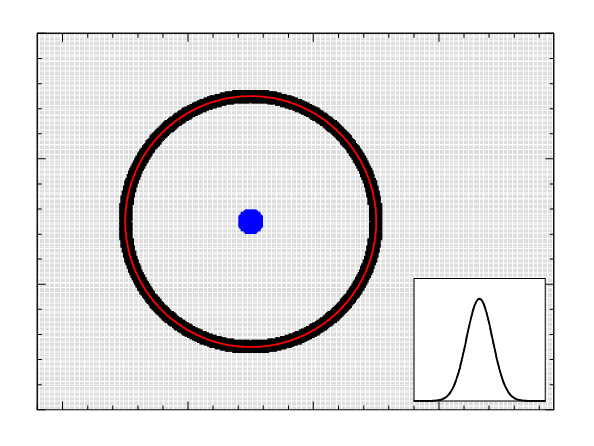
\includegraphics[width=0.45\columnwidth]{images/misc/slice000.png}%
    }\hfill
    \subfloat[]{
      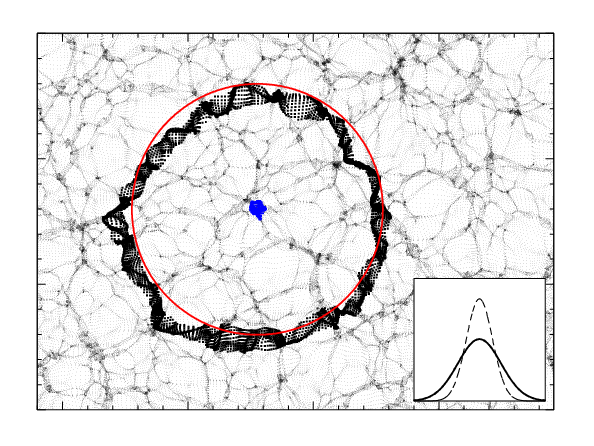
\includegraphics[width=0.45\columnwidth]{images/misc/slice040.png}%
    }\hfill
    \subfloat[]{
      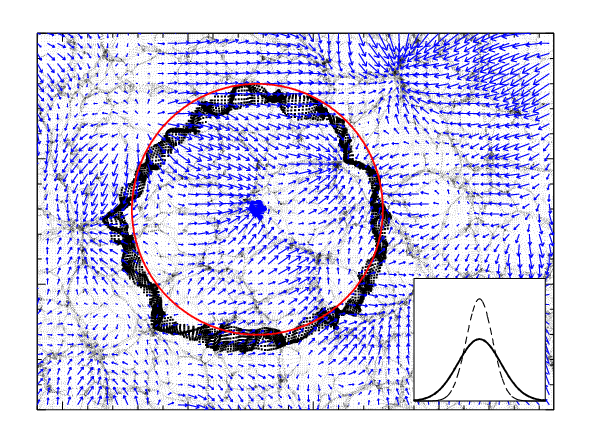
\includegraphics[width=0.45\columnwidth]{images/misc/vector040.png}%
    }\hfill
    \subfloat[]{
      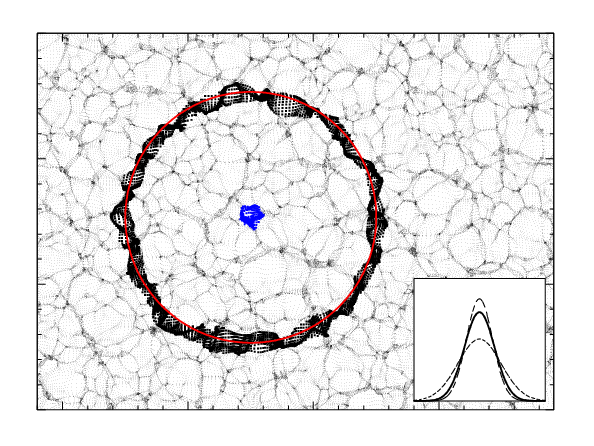
\includegraphics[width=0.45\columnwidth]{images/misc/recon040.png}%
    }\hfill
    
    \caption{
      \setstretch{1.0}
      \small
    An illustration taken from~\cite{2012MNRAS.427.2132P}, showing how the acoustic scale is distorted by non-linear effects and then reconstructed. (a) In the early Universe, the density field was very smooth. The acoustic feature is marked with a ring of radius $150Mpc$, and the distance between the centroid (blue point) and the radially distributed black points is represented by a Gaussian. (b) In the late Universe, non-linear effects move the points on the acoustic scale from their original positions (still represented by the red circle). This can be seen as a broadening of the radial distribution (dashed line is the original). The evolution here was modelled using the Zel'dovich approximation. (c) The Lagrangian displacement field (blue arrows) is calculated. The concept behind reconstruction techniques is to estimate the displacement field in order to move the particles back to their original position. The field was smoothed using a Gaussian filter. (d) The particles were moved back along the displacement field, and a clear improvement can be seen. The solid line marks the reconstructed radial distribution, the dashed line represents the primordial distribution, and the dotted line is the late time distribution before reconstruction. In this case the reconstruction is not perfect because of the Gaussian filter, which was used to mimic a real scenario. Note that this was done just for illustration purposes, and actual reconstruction methods are more complex.
    }
    
\label{fig:3}
\end{figure}



